\documentclass[12pt, a4paper]{article}
\usepackage[utf8]{inputenc}
\usepackage{amsmath}
\usepackage{amsfonts}
\usepackage{amssymb}
\usepackage{graphicx}
\usepackage{caption}
\usepackage{subcaption}
\usepackage{sidecap}
\author{MORAES, FELIPE}
\title{Fundamentals of STDP based recurrent assembly networks}

\newtheorem{theorem}{Theorem}[section]
\newtheorem{lemma}[theorem]{Lemma}
\newtheorem{proposition}[theorem]{Proposition}
\newtheorem{corollary}[theorem]{Corollary}

\newenvironment{proof}[1][Proof]{\begin{trivlist}
\item[\hskip \labelsep {\bfseries #1}]}{\end{trivlist}}
\newenvironment{definition}[1][Definition]{\begin{trivlist}
\item[\hskip \labelsep {\bfseries #1}]}{\end{trivlist}}
\newenvironment{example}[1][Example]{\begin{trivlist}
\item[\hskip \labelsep {\bfseries #1}]}{\end{trivlist}}
\newenvironment{remark}[1][Remark]{\begin{trivlist}
\item[\hskip \labelsep {\bfseries #1}]}{\end{trivlist}}

\newcommand{\qed}{\nobreak \ifvmode \relax \else
      \ifdim\lastskip<1.5em \hskip-\lastskip
      \hskip1.5em plus0em minus0.5em \fi \nobreak
      \vrule height0.75em width0.5em depth0.25em\fi}

\renewcommand{\figurename}{Figura}

\begin{document}

\begin{center}
{\huge TRABALHO PRÁTICO 2: Montador}
\textit{Felipe Moraes Gomes - felipemoraes@dcc.ufmg.br}
\end{center}
\section{Introdução e Definição do Trabalho}
Este trabalho descreve a implementação e operação de um montador para uma linguagem assembly hipotética, baseada no conjunto de instruções do RISC. A máquina virtual recebe como entrada um arquivo de texto, contendo o código a ser montado, e alguns parâmetros de execução, que ele então usa para construir o executável.

O restante deste documento está organizado da seguinte forma: A 2\textsuperscript{a} seção trata da implementação do montador e de sua organização no código; A 3\textsuperscript{a} seção resume o formato de execução, entrada e saída do programa; A 4\textsuperscript{a} seção contém os testes realizados; A 5\textsuperscript{a} seção conclui o trabalho. Após isso, é colocado um apêndice contendo uma listagem dos arquivos do projeto. 

\section{Implementação e Organização}

O montador abre o arquivo de código especificado e monta o executável em dois passes. Primeiramente, o arquivo é lido com o intuito de criar a tabela de símbolos. Em seguida, o arquivo é relido e traduzido, gerando o executável. 

A verificação sintática foi implementado para auxiliar na depuração dos programas de teste desenvolvidos. O montador é representado por procedimentos do algoritmo principal, cujos componentes principais são delineadas a seguir.

\subsection{Dados e Variáveis}

\emph{Estruturas de Dados} define várias estruturas de dados, 

\begin{itemize}
	\item \emph{TipoLista symbol\_table}: Tabela de símbolos que associa um label (string) com o ILC referente à aquele local. 
	\item \emph{TipoLista opcode\_table}: Tabela de instruções que associa a string que identifica a instrução no assembly com seu respectivo índice no código de máquina. As pseudo-instruções \emph{WORD} e \emph{END} foram atribuídos os valores 22 e 23, respectivamente (muito embora estes valores são usados somente internamente, ausentando-se do executável). As demais instruções são codificadas conforme a especificação.
	\item \emph{TipoLIsta size\_table}: Tabela de instruções que associa o índice da instrução com seu tamanho.
\end{itemize}

\subsection{Procedimentos e Funções}

\begin{itemize}
	\item \emph{char* readline()}: Lê uma linha do arquivo fonte e a retorna.
	\item \emph{char* next\_word}: Extrai a próxima palavra de uma linha, apagando ela na linha original, retorna nulo caso linha vazia, ou somente comentários.
	\item \emph{void Decode()}: Recebe uma linha do arquivo de código fonte, e a decodifica, retornando o índice da instrução (usando \emph{opcode\_table}), e, se for o caso, o label da linha e o número e valor dos operandos. Caso seja encontrada uma instrução desconhecida ele segue para frente.
	\item \emph{void Primeiro\_Passo()}: Abre o arquivo fonte, e efetua a primeira passada, construindo a tabela de símbolos. Para tal, \emph{readline()} é chamado continuamente até que \emph{END} seja encontrado. O ILC é simulado a cada instrução e, se na linha houver um label, é associado a ele pela lista \emph{symbol\_table}. 
	\item \emph{void Segundo\_Passo()}: Efetua a segunda passada, fazendo a tradução e escrevendo o executável. Para tal, \emph{Decode} é chamado continuamente até que \emph{END} seja encontrado. Cada instrução decodificada é traduzida e colocado na saída, substituindo os labels das referências de memória pelo PC associado (\emph{symbol\_table}), observando que no caso da pseudo-instrução \emph{WORD}, somente o operando é usado.  
	\item Os restantes das funções, são de descrição desnecessária, uma vez que é usada continuamente em muitas disciplinas do curso.
\end{itemize}

\subsection{Fluxo de Execução}

O programa inicialmente lê os parametros passados a ele, verificando seu formato. Caso correto, ele constrói a tabela de instruções (\emph{opcode\_table}). Em seguida, o arquivo contendo o código fonte é aberto, e sua tabela de símbolos é construída (primeiro passe). Finalmente, \emph{Segundo\_Passo()} é chamado, que efetua a tradução, e monta o executável. Ao retornar, o programa imprime a tabela de símbolos (se o mesmo foi especificado) e conclui sua execução.

\section{Controle \& IO}

\subsection{Execução e Compilação do Simulador}

O programa pode ser compilado através do g++, pelo utilitário \emph{make}, usando o makefile providenciado. Uma vez compilado, chamadas devem seguir o formato:

\begin{center}
\emph{./montador input.amk output.mk `s'{\tt{|}}`v'}
\end{center}

Onde `s' especifica que a saída deve ser simples (somente se for detectado um erro de sintaxe), e `v' especifica que o programa deve também imprimir a tabela de símbolos. \emph{input} é o nome do arquivo de entrada que contém o código assembly a ser traduzido, e \emph{output} é o nome do arquivo executável gerado pelo montador.

\subsection{Formato dos Arquivos de Entrada e Saída}

Cada linha dos programas em assembly devem seguir o formato:

\begin{center}
[{\tt<}label{\tt>}:] {\tt<}instrução{\tt>} {\tt<}operando1{\tt>} {\tt<}operando2{\tt>} [; comentário]
\end{center}

Onde \emph{label} e \emph{comentário} são opcionais, porém devendo ser devidamente delimitados (o sufixo ``:'' para o label e o prefixo ``;'' para o comentário), e o tipo e quantidade dos operandos é dependente da instrução.

Os programas gerados são codificados em um arquivo de texto, onde cada linha contém exatamente um \emph{WORD}, que representa um dado ou uma instrução, segundo a codificação delimitada na especificação.

\section{Testes}

\begin{figure}
\centering
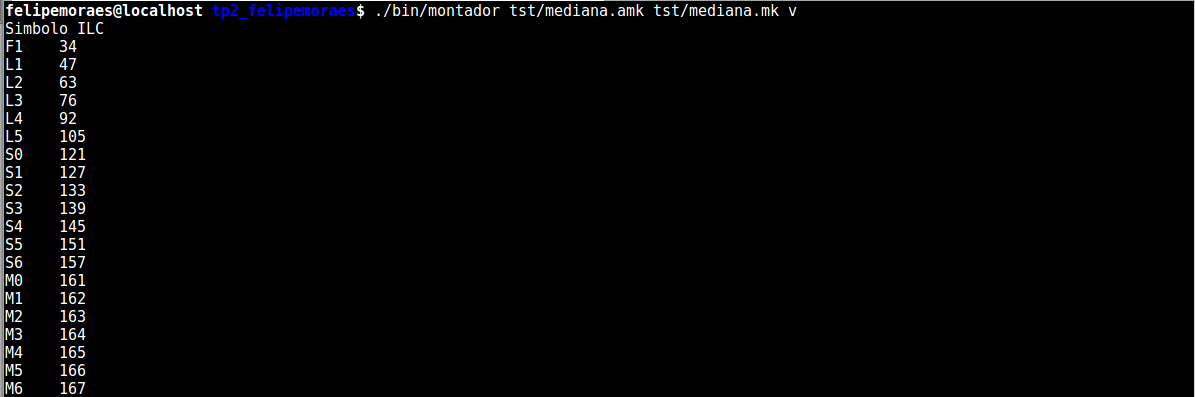
\includegraphics[width=0.9\textwidth]{RuntimeScreencap1.png}
\caption{Montagem dos testes - Teste Mediana}
\label{FigureExecution1}
\end{figure}

\begin{figure}
\centering
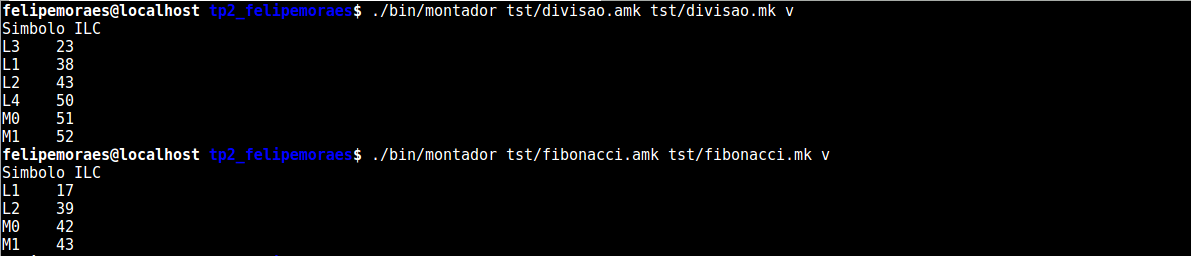
\includegraphics[width=0.9\textwidth]{RuntimeScreencap2.png}
\caption{Montagem dos testes - Teste Divisão e Fibonacci}
\label{FigureExecution2}
\end{figure}

Múltiplos programas foram montados, de forma a obter cobertura total do código. Os testes podem ser executados no emulador. As tabelas de símbolos obtidas durante a tradução de cada programa são ilustradas na Fig. \ref{FigureExecution1} e \ref{FigureExecution2}.

\begin{itemize}
	\item \emph{Divisão força bruta (divisao.amk):} Faz a divisão força bruta de dois números (passados como parâmetros), e imprime o quociente e o resto obtido. O tratamento de valores negativos foi feito de tal forma que a soma do resto com o produto do quociente com o divisor sempre desse o numerador (com $0 \leq resto < |Divisor|$).
	\item \emph{Fibonacci (fibonacci.amk)}: Imprime o enésimo número da sequência fibonacci, onde \emph{N} é passado como parâmetro.
	\item \emph{Mediana de 7 (mediana.amk)}: Dado um conjunto de 7 números (lidos do terminal), imprime sua mediana.
\end{itemize}

\section{Conclusão}

O montador é eficaz em lidar com programas escritos neste conjunto de instruções, podendo ser usado não só para traduzi-los mas também para adequadamente depurar erros de sintaxe.

A execução do trabalho transcorreu sem maiores dificuldades, e os resultados obtidos correspondem ao esperado.

\appendix
\section{Apêndice}
\subsection{Listagem de Arquivos}
\begin{itemize}
	\item Código Fonte:
	\begin{itemize}
		\item \emph{src/main.c:} Interpreta os parâmetros de entrada e controla o fluxo do programa (Seção 2.3).
		\item \emph{src/assembler.c, src/assembler.h:} Implementa o montador (Seção 2.1 e 2.2).
		\item \emph{src/io.c, src/io.h:} Implementa funções de entrada e saida.
		\item \emph{src/lista.c, src/lista.h:} Implementa a TAD lista encadeada.
		\item \emph{src/Makefile:} Makefile para facilitar a compilação do programa (Seção 3.1).
	\end{itemize}
	\item Testes:
	\begin{itemize}
		\item \emph{tst/divisao.amk; tst/divisao.mk:} (Seção 4 item 1).
		\item \emph{tst/fibonacci.amk; tst/fibonacci.mk:} (Seção 4 item 2).
		\item \emph{tst/mediana.amk; tst/mediana.mk:} (Seção 4 item 3).
	\end{itemize}
	
\end{itemize}

\end{document}
